\documentclass{beamer}

\usepackage{fontspec}
\usepackage{booktabs}
\usepackage[ngerman]{babel}
\usepackage{verbatim}
\usepackage{fancyvrb}
\usepackage{listings}
\usepackage{csquotes}

\usepackage{tikz}
\tikzset{every picture/.style={line width=0.2mm}}
\usetikzlibrary{calc}

\usepackage[european,s traightvoltages, RPvoltages, americanresistor, americaninductors]{circuitikz}

\usepackage{biblatex}
\addbibresource{bib.bib}

\usetheme{Berlin}
\usecolortheme{beaver}

\usefonttheme{professionalfonts} % using non standard fonts for beamer
\usefonttheme{serif} % default family is serif
\setmainfont{Liberation Serif}


\lstset{
    basicstyle=\ttfamily,
    language=[LaTeX]TeX,
}



\title{Einf\"uhrung in \LaTeX}
\author{Daniel Renschler}
\date{17. Juli 2023}


\begin{document}


\begin{frame}
    \titlepage 
\end{frame}


\begin{frame}
    \tableofcontents
\end{frame}


\section{\LaTeX?}
\begin{frame}{Geschichte}
    \begin{columns}
        \column{0.5\textwidth}


    \begin{itemize}
        \item Donald Knuth hat 1977-1986 \TeX gemacht, da er die typografische Qualit\"at seiner B\"ucher nicht gut fand. (The Art of Computer Programming)

    \end{itemize}
        
        \hfill
        \column{0.5\textwidth}
        \begin{figure}[htpb]
            \centering
            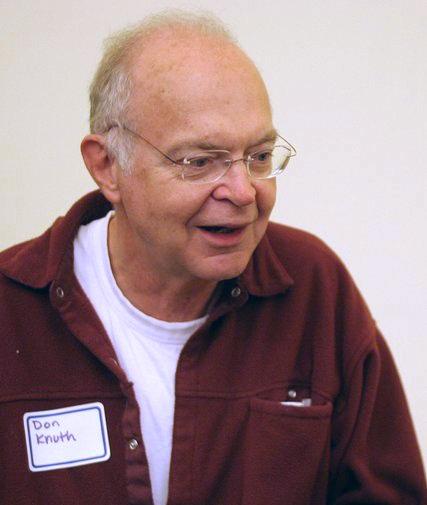
\includegraphics[width=0.7\textwidth]{./figs/tex-knuth.jpg}
        \end{figure}
    \end{columns}
\end{frame}

\begin{frame}{Was ist \LaTeX?}
    \begin{itemize}
        \item Textsatzystem.
        \item Erm\"oglicht Erstellen von Dokumenten.
        \item Beliebt im Akademischen Bereich/Wissenschaft.
        \item Erstellt hochwertige PDF Ausgabe.
    \end{itemize}
    
\end{frame}



\begin{frame}{Warum \LaTeX?}
    \begin{itemize}
        \item Ist sehr intuitiv.
        \item Sehr extensiv mit packages.
        \item K\"ummert sich um viel von alleine
        \item Man muss sich nicht mit Typografie und Vergleichbarem vertraut machen\footnote{Es funktioniert einfach und sieht gut aus.}.
        \item Macht spa\ss
    \end{itemize}
\end{frame}



\begin{frame}{Warum nicht Word? (oder andere WYSIWYG\footnote{WYSIWYG = What you see is what you get} software)}
    \begin{itemize}
        \item Word macht es schwerer \"Anderungen an gro\ss{}en Dokumenten vorzunehmen.
        \item Bibliografien werden nicht automatisch gemacht, auch Zitierstil nachtr\"aglich \"anderbar.
        \item Seitenzahlen, Referenzen, etc. werden nicht automatisch erzeugt.
        \item \textit{kann man nicht in Vim benutzen.}
    \end{itemize}
    
\end{frame}




\begin{frame}{Nutzzwecke}

    \begin{itemize}
        \item Ausarbeitungen/Laborberichte
        \item Pr\"asentationen
        \item Dokumente
        \item Lebenslauf
        \item B\"ucher
    \end{itemize}
\end{frame}




\section{Beispiele}
\begin{frame}{Berichte}
    \begin{itemize}
        \item Laborberichte 
    \end{itemize}
    \begin{figure}[htpb]
        \centering
        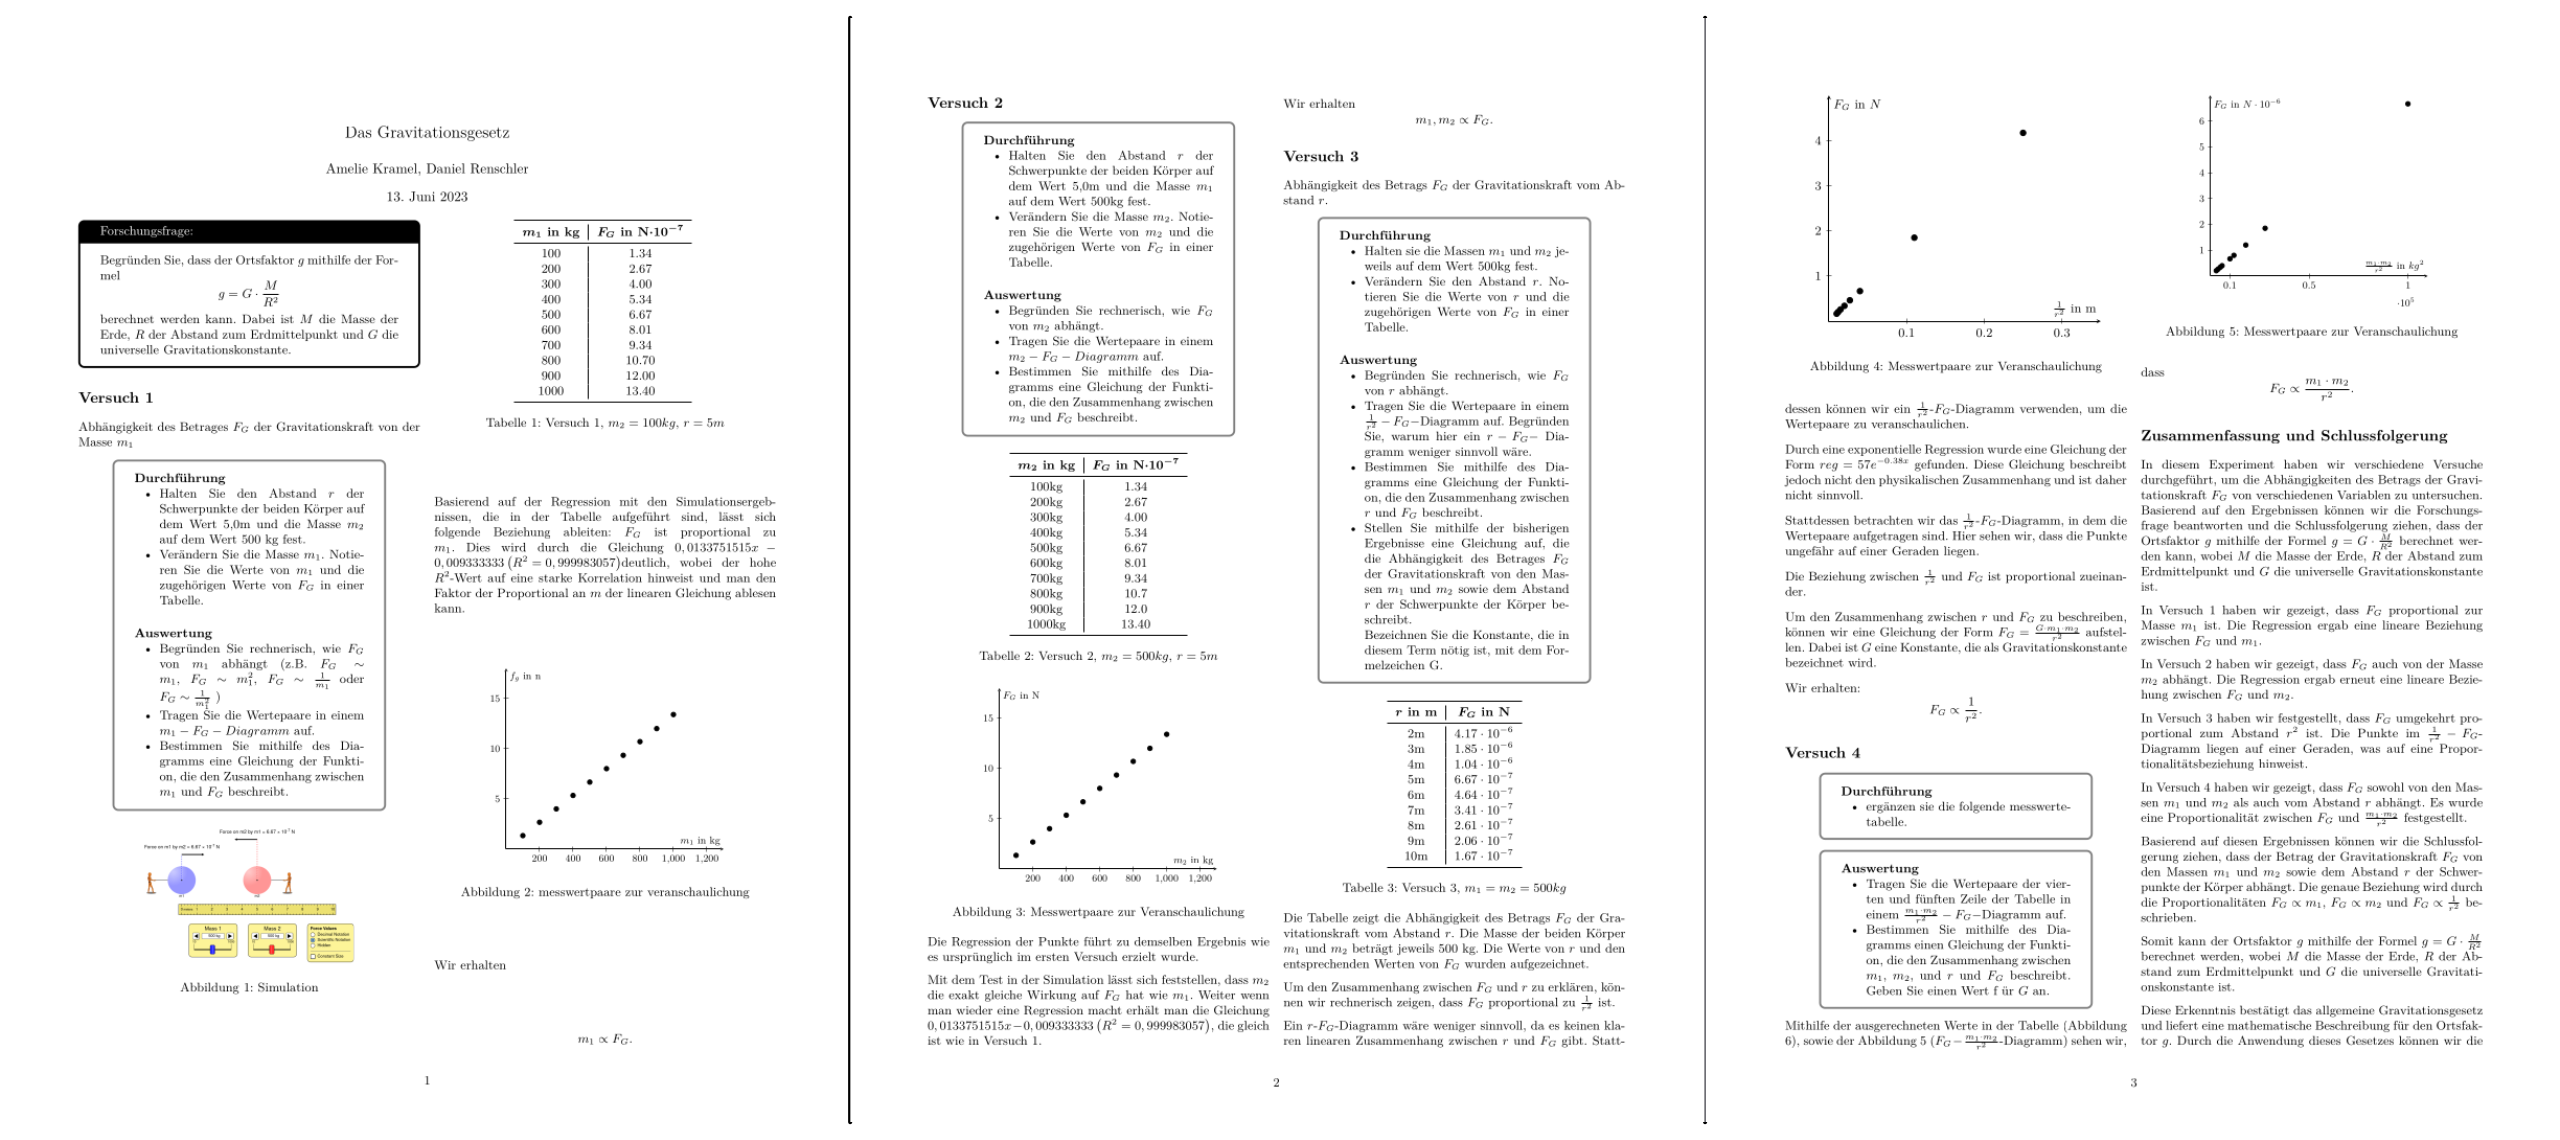
\includegraphics[width=1\textwidth]{./figs/am stueck.png}
        \caption{Laborprotokoll Gravitationsgesetz}
        \label{fig:}
    \end{figure}
\end{frame}



\begin{frame}{Paper}
    \begin{figure}[htpb]
        \centering
        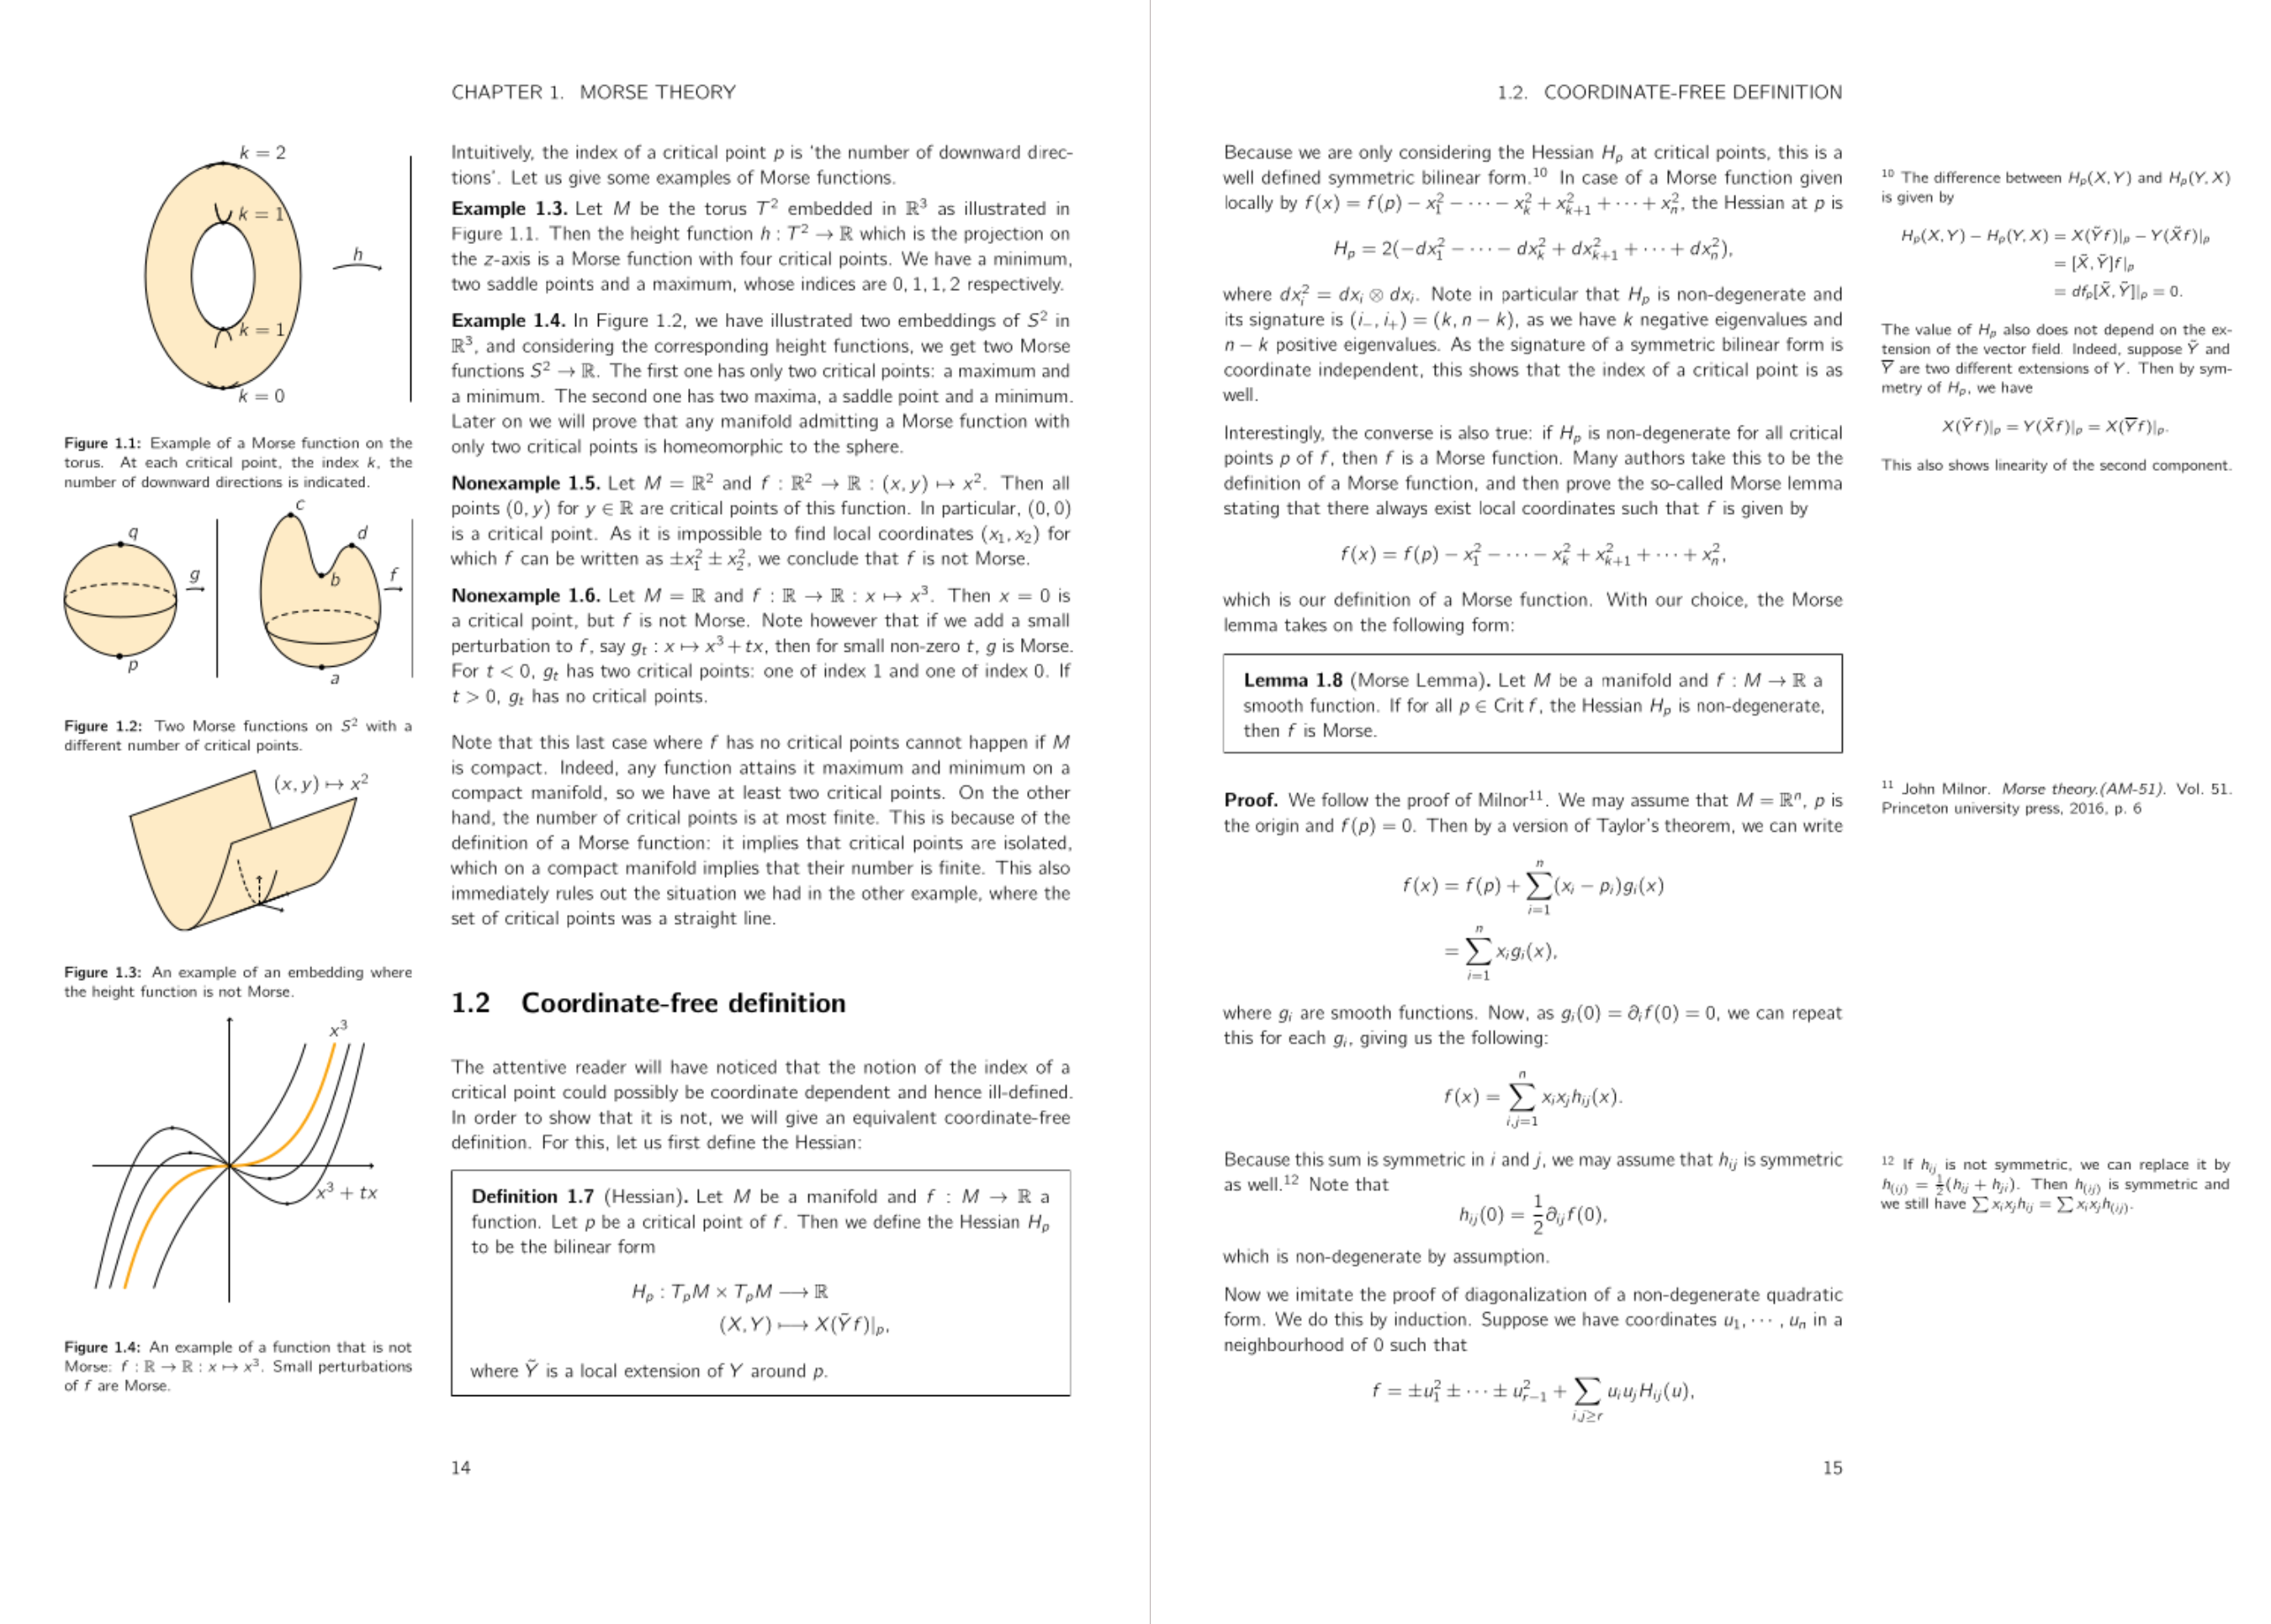
\includegraphics[width=0.7\textwidth]{./figs/example-paper.png}
        \caption{Auszug einer Masterarbeit \"uber Morse Theory}
    \end{figure}
\end{frame}


\begin{frame}{Beispiel 1}


Beispiele:
\begin{itemize}
    \item Irgendwas mit Euler \cite{baranek2023randomized}
        \[ \mathcal{L} = \frac{\partial}{\partial t}+ \frac{1}{2}\sum_{k=1}^{m}\frac{\partial^2}{\partial y_{k}^2} .\] 
\end{itemize}


\begin{itemize}
    \item Analysis Aufgabe: 
        \[ \lim_{x\to \int_0^{\infty} \sqrt{t}e^{-t}dt}\left( \left( \sum_{n=0}^{\infty}\frac{x^{4n_4}}{(2n+1)(4n+3)(4n+4)} \right)''  \right) .\] 
\end{itemize}
\end{frame}

    



\begin{frame}{Toeplitz Matrix}
    \[ A=\begin{bmatrix}
            a_0 & a_{-1} & a_{-2} & \ldots & \ldots  &a_{-n+1}  \\
            a_1 & a_0  & a_{-1} &  \ddots   &  &  \vdots \\
            a_2 & a_1 & \ddots  & \ddots & \ddots& \vdots \\ 
            \vdots &  \ddots & \ddots &   \ddots  & a_{-1} & a_{-2}\\
            \vdots &         & \ddots & a_1 & a_0 &  a_{-1} \\
            a_{n-1} &  \ldots & \ldots & a_2 & a_1 & a_0
        \end{bmatrix} .\] 
\end{frame}



\begin{frame}{Physik Beispiel}
    Sequential Quantum Circuits as Maps between Gapped Phases.\cite{chen2023sequential}
    \begin{align*}
        \frac{1}{|G|}\sum_g X^g_i &\to \sum_h T^h_{i-1}T^h_i, \quad i=2,\ldots,N,  \\
        \frac{1}{|G|} \sum_g X_1^g &\to \frac{1}{|G|} \sum_{h,h'}e^{-\frac{2\pi i}{|G|}(h'-h)g}T_1^hT^{h'}_N \prod^N_{i=1}X_i^g,  \\
        \sum_h T^h_i T^h_{i+1} &\to \frac{1}{|G|} \sum_g X_i^g, i=2,\ldots,N  \\
        \sum_h T^h_1 T^h_2 &\to \frac{1}{|G|} \sum_g X_1^g \prod_{i=1}^N X_i^g.
    \end{align*}
\end{frame}




\begin{frame}{Abbildungen (tikz)}

\begin{tikzpicture}
	\begin{circuitikz}[scale=0.7]
		\ctikzset{voltage/american plus/.initial={}, voltage/american minus/.initial={}}
	
		%Coordinates
		\node[njfet] (Q) at (5,3.5) {};
		
		% Circuit
		\draw
		
		(Q.S) node[shift={(-0.3,0)}] {$S$} to[R, l^=$R_3$, *-*] ++(0,-2.5) node[ground] (GR) {}
		
		(Q.D) node[shift={(-0.3,0)}] {$D$} to[R, l^=$R_2$, *-] ++(0,2.8) node[vcc] {$+V_{DD}$}
		(Q.D) to[C, l^=$C_2$] ++(4,0) -- ++(0,-1.35) node (D') {} 
			  to[open, v=$v_o$, o-o, american] ++(0,-1.3) -- (GR -| D') -- (GR)
		
		(Q.G) node[shift={(0,0.4)}] {$G$} -- ++(-1,0) node[inner sep=0, outer sep=-1] (G') {} to[R, l_=$R_1$] (GR -| G')
		(G') to[C, l_=$C_1$] ++(-3,0) node (G'') {};
		
		\draw (GR) -- (GR -| G'');
		
		\draw[dashed]
		(Q.S) -- ++(2,0) to[curved capacitor, l^=$C_3$, -*] ++(0,-2.5)
		(G'') to[sV, l_=$v_{in}$, *-*] (G'' |- GR);
		
	\end{circuitikz}
	\end{tikzpicture}

\end{frame}



\section{Syntax \& etc.}
\begin{frame}{Syntax}

\begin{itemize}
    \item Commands beginnen mit \textbackslash{}, nicht zu verwechseln mit \Verb|/|
    \item Umgebungen (environments) beginnen und enden immmer gleich, man kann/muss nesten.
\end{itemize}


\end{frame}



\begin{frame}[fragile]
    \frametitle{Struktur}
Struktur die in jedem Dokument eingehalten werden muss:
    
\begin{lstlisting}
\documentclass{article}
\usepackage{tikz} % Fuer Zeichnungen
\usepackage{amsmath} % Fuer mathematische Symbole

\begin{document}
    
\end{document}
\end{lstlisting}

\end{frame}



\begin{frame}{Documentclasses}
   Gibt viele, die wichtigsten sind: 
   \begin{itemize}
        \item \Verb|article|: ``normale Klasse'' Titel ist auf erster Seite
        \item \Verb|report|:  Titel hat eigene Seitenzahlen
        \item \Verb|beamer|: F\"ur Pr\"asentationen (diese z.B.)
        \item Andere sind: \Verb|book|, \Verb|letter|, etc.
   \end{itemize}
\end{frame}



\begin{frame}{Sections}
Es gibt verschiedene an Sections.

\begin{itemize}
    \item section
    \item subsection
    \item subsubsection
\end{itemize}

Diese werden dann z.B. in Inhaltsverzeichnissen angezeigt und sich untergeordnet.

\begin{itemize}
    \item Section
        \begin{itemize}
            \item subsection
                \begin{itemize}
                    \item subsubsection
                \end{itemize}
        \end{itemize}
\end{itemize}
\end{frame}




\begin{frame}[fragile]{Fu\ss{}noten und Bibliografien}

Eine Fu\ss{}note macht man:
\begin{lstlisting}
\footnote{Fußnoteninhalt}
\end{lstlisting}

Eine Zitat macht man:
\begin{lstlisting}
\cite{Zitat}
\end{lstlisting}

Eine Bibliografie macht man:
\begin{lstlisting}
\printbibliography
\end{lstlisting}

\vfill

Fu\ss{}note\footnote{Fußnoteninhalt}

Zitat \cite{smith2017}

\end{frame}



\begin{frame}{Math environments}
    Mathe wird in math-environments geschrieben.
    \begin{itemize}
        \item inline math, z.B. $f(x)=x^2$: \lstinline{$ ... $}
        \item display-math, z.b. \[
            \frac{1}{|G|}\sum_g X^g_i \]
         mit: \textbackslash [ ... \textbackslash ] 

         \item Gleichungen, mit einem align environment.
    \end{itemize}


\end{frame}


\begin{frame}{Mathe 1}
    \begin{itemize}
        \item superscript: \lstinline{^}, bzw. \lstinline{^\{\}} 
            \begin{itemize}
                \item $e^x$: \lstinline{e^x}
            \end{itemize}
        \item subscript: \lstinline{_}, bzw. \lstinline{_\{\}} 
            \begin{itemize}
                \item $e_x$: \lstinline{e_x}
            \end{itemize}
        \item Br\"uche: \textbackslash\lstinline{frac\{\}\{\}}
            \begin{itemize}
                \item $\frac{a}{b}$, $ \frac{1}{\frac{2}{\frac{3}{4}}}$ \[
                    \frac{1}{\frac{1}{\frac{1}{\frac{1}{2}2}2}2} .\] 
            \end{itemize}
    \end{itemize}
\end{frame}

\begin{frame}{Mathe 2}

\begin{itemize}
    \item Integral: \textbackslash\lstinline{int_0^\{}\textbackslash\lstinline{pi\}}\[ \int_{0}^{\pi} \] 
    \item Summe: \textbackslash\lstinline{sum_0^1}\[ \sum_{0}^{1},\ \prod^1_0 \]
\end{itemize}



\end{frame}



\section{Anderes}

\begin{frame}{Aus gestalterischer Sicht}
    Im Vergleich zu Affinity Publisher

    \begin{table}[htpb]
        \centering
        \begin{tabular}{p{0.4\textwidth}|p{0.4\textwidth}}
            Publisher & \LaTeX \\
            \toprule
            Wird unübersichtlich, wenn man nicht genau weiß, was man macht. & Wird auf größeres Dokument nicht unübersichtlich.\\
            \midrule
            Man muss alles grafisch anordnen. & Sachen sind da, wo sie hingehören.\\
        \end{tabular}
    \end{table}


\end{frame}


\begin{frame}{Wie man es benutzt}
    \begin{itemize}
        \item Arch-basiert: \Verb|pacman -S texlive-basic|
        \item Debian-basiert: \Verb|apt-get install texlive-full|
        \item MacOS: \Verb|MacTeX|
        \item Windows: \Verb|MiKTeX|
        \item Online: Overleaf
    \end{itemize}
\end{frame}




\begin{frame}{Weitere Resourcen}
    \begin{itemize}
        \item diese Pr\"asentation: \url{https://github.com/d-rens/LaTeX-Einfuehrung/}
        \item \LaTeX\ Tutorials, von Luke Smith
        \item Overleaf Tutorials
        \item ``The \TeX book", von Donald E. Knuth
    \end{itemize}
    
\end{frame}




\begin{frame}{Literatur}
    \printbibliography
    
\end{frame}





\end{document}
